\documentclass[10pt]{article}

\usepackage[margin=0.82in]{geometry}
\usepackage[T1]{fontenc}
\usepackage{lmodern}
\usepackage{microtype}
\usepackage{amsmath,amssymb}
\usepackage{graphicx}
\usepackage{booktabs}
\usepackage{tabularx}
\usepackage{array}
\usepackage{multirow}
\usepackage{siunitx}
\usepackage{enumitem}
\usepackage{caption}
\usepackage{subcaption}
\usepackage{float}
\usepackage{tikz}
\usetikzlibrary{arrows.meta,positioning,fit}
\usepackage[numbers,sort&compress]{natbib}
\usepackage{xcolor}
\usepackage{fancyhdr}
\usepackage[hidelinks]{hyperref}

\definecolor{jewelblue}{HTML}{2457A6}
\definecolor{jewelgold}{HTML}{B87B16}
\definecolor{softgray}{HTML}{F3F5F7}
\hypersetup{
  colorlinks=true,
  linkcolor=jewelblue,
  citecolor=jewelblue,
  urlcolor=jewelblue,
  pdftitle={Jewels: Toward Text-Conditioned, Streamable, and Locally Editable Video as Space-Time Gaussian Fields},
  pdfauthor={The Jewels Project}
}
\sisetup{detect-all,table-number-alignment=center}
\captionsetup{font=small,labelfont=bf}
\setlist{nosep,leftmargin=*}
\setlength{\parskip}{0.35em}
\setlength{\parindent}{0pt}
\setlength{\tabcolsep}{5pt}
\emergencystretch=2em

\pagestyle{fancy}
\fancyhf{}
\lhead{Jewels technical report}
\rhead{August 2026}
\cfoot{\thepage}
\renewcommand{\headrulewidth}{0.4pt}

\newcommand{\jewels}{\textsc{Jewels}}
\newcommand{\uvt}{(u,v,t)}
\newcommand{\R}{\mathbb{R}}
\newcommand{\todoresult}{\textcolor{jewelgold}{\textbf{open}}}

\title{\vspace{-1.5em}\textbf{Jewels: Toward Text-Conditioned, Streamable, and\\Locally Editable Video as Space-Time Gaussian Fields}}
\author{The Jewels Project}
\date{Technical report -- August 12, 2026}

\begin{document}
\maketitle
\vspace{-1.2em}
\begin{center}
\fcolorbox{jewelblue}{softgray}{\parbox{0.92\linewidth}{\small
\textbf{Status.} This is a progress report, not a benchmark or a claim of completed text-to-video generation.
It separates established results, failed controls, and hypotheses still under test.}}
\end{center}

\begin{abstract}
We investigate whether ordinary RGB video can be generated and edited as an explicit field of
anisotropic Gaussian primitives in normalized image-time coordinates rather than as a sequence of
pixel frames. Each primitive, or \emph{jewel}, occupies a volume in \uvt, carries opacity and a
linear color field, and may tilt through time so that motion is represented by oriented space-time
support. A deterministic additive renderer turns the set into frames. The longer-term model emits
new jewels in overlapping time windows, retains persistent jewels by stable identity, and repairs
only dirty latent cells after a user moves selected primitives.

This report consolidates the feasibility evidence to date. Synthetic tubes reconstruct at about
\SI{55}{dB}; four finalized 96-frame UCF-101 fields with 120k jewels replay at a mean
\SI{32.28}{dB}. A density audit shows that raw jewel count is misleading: doubling a UCF field from
45k to 90k isotropically increases effective per-frame contributors by only 30.3\% and lowers
full-volume PSNR by \SI{1.07}{dB}, motivating temporal-preserving spatial densification. A local
$32^3\!\times\!24$ tokenizer is the first held-out configuration to preserve small pedestrians;
a train-only $2^3$ PCA hierarchy reduces it to $16^3\!\times\!96$ with a \SI{0.224}{dB} penalty.
An axial rectified-flow prior beats retrieval and mean-collapse distribution baselines but does not
use its semantic condition. Conversely, a cell-local prefix model reduces future-birth feature
error by 62.7\% against a disjoint shuffled-prefix control and renders at \SI{19.87}{dB} versus
\SI{7.30}{dB}. Edit planning and masked sampling preserve every clean latent exactly, although the
repaired region remains blurry. A four-class direct prompt model changes held-out birth statistics
but produces washed-out action geometry. Exact target topology improves its mean field PSNR by only
\SI{0.172}{dB}, rejecting count prediction as the primary cause. Oracle-topology stochastic flow
recovers edge energy without coherent objects; adding the true future as a \(24\times40\) guide
raises held-out rendering from 14.232 to \SI{16.555}{dB} and from 59.8\% to 90.5\% of target edge
energy. This privileged control selects a semantic-video-scaffold-to-jewel architecture; it is not
a prompt-only generation result. Official distilled LTX-2.3 then produces all 16 balanced prompt
scaffolds. Four density-matched 49-frame/72k-jewel reconstructions replay at
\SIrange{28.18}{35.16}{dB}, averaging 5,966 effective contributors/frame. Token-only multiscale,
raster-plus-token, and two raster-guide render-loss controls fail to dominate the original guide.
The selected UCF-trained realizer then passes a predeclared cross-domain gate on the four unseen
LTX scaffolds: guided samples reach 15.342 dB/0.6942 SSIM versus 13.777 dB/0.4160 for deterministic
continuation, move contrast from 0.426 to 0.743 and edge energy from 0.486 to 0.830, retain 99.08\%
birth-cell adherence, and preserve a recognizable primary action in three of four classes. Correct
and shuffled text remain tied once the true LTX video guide is present. The result therefore
validates privileged scaffold-to-jewel transfer, not free prompt-only jewel generation. A new
0.88M-parameter scaffold/carry topology head then removes fitted birth cells, counts, and ranks for
one held-out LTX continuation stride. Correct-scaffold slot F1 is 0.6636 versus 0.6092 shuffled,
0.6091 null, and 0.6222 train mean. When the frozen flow synthesizes every predicted rank, learned
topology reaches 15.464 dB/0.6967 SSIM versus 15.492 dB/0.6997 with oracle topology, predicts
99.68\% of the birth budget, averages 5,822 effective contributors/frame, and copies carried
features with zero error. This passes autonomous topology and density for one continuation; the
initial field and multi-stride generated carry remain open.

Gaussian reconstruction of video is not new: VeGaS, GSVC, GaussianVideo, GaRV, and related work
predate this project. The research opportunity evaluated here is narrower: a corpus-level
generative distribution that directly emits persistent, editable 2D-video space-time Gaussian
fields. Because the field is a representation rather than a sampling objective, it can in
principle be generated by flow matching, diffusion, or next-token prediction. Its hierarchy also
suggests a structured multimodal event language in which text, persistent visual state, and edit
operations share one sequence. We state these as provisional systems hypotheses, not priority
claims.
\end{abstract}

\section{Introduction}

Pixel video models repeatedly synthesize dense frames and must learn temporal coherence through
architecture, loss, or data. \jewels{} asks whether coherence can instead be partly structural. We
treat a video as a continuous three-dimensional signal over horizontal position, vertical position,
and time. A moving visual element can then be represented by a Gaussian tube whose principal axis
leans through time. The model is explicit: primitives can be selected, moved, recolored, carried
between generation windows, culled at multiple levels of detail, and rendered at arbitrary times.

The intended system is not merely a codec. It is a text-to-video model whose native output is an
editable space-time field. After generation, a viewer sees the video as a parallelepiped, drags a
cursor through it, moves one or many jewels, and asks the model to resample only the vacated and
destination neighborhoods. Untouched regions are hard constraints rather than soft conditioning.

The project has progressed through a sequence of falsifiable gates:

\begin{enumerate}
  \item demonstrate that anisotropic space-time primitives can fit motion and ordinary video;
  \item measure whether fitted sets are canonical enough for a shared generative model;
  \item raise effective splat density without destroying temporal persistence;
  \item learn a deterministic, count-aware local bottleneck for dense fields;
  \item generate hierarchical latents with tractable attention;
  \item prove exact edit locality and overlap-conditioned continuation; and
  \item introduce text only after a leakage-safe prompt corpus exists.
\end{enumerate}

Our contributions are therefore empirical and architectural rather than a completed generative
benchmark. We report (i) an additive \uvt{} Gaussian representation and gauge-free field features,
(ii) density and tokenizer experiments that identify what preserves small moving subjects,
(iii) controlled evidence that spatially aligned prefix context is essential for continuation,
(iv) an edit/inpaint formulation with exact clean-region preservation, and (v) explicit negative
results that bound what remains unproved. We further isolate deterministic conditional averaging as
the current washout mechanism and show that a low-resolution semantic scaffold can recover global
layout in stochastic jewel realization and transfer from UCF training to unseen prompt-generated
LTX videos without mark-model retraining. We then replace fitted continuation topology with
scaffold/carry-predicted counts and show that the frozen realizer remains within 0.028 dB of its
oracle-topology control at the intended effective density. We additionally articulate two falsifiable systems
hypotheses: that explicit persistent fields offer interaction properties unavailable from an opaque
raster latent alone, and that a hierarchical field can serve as a multimodal visual event language.

\begin{figure}[H]
\centering
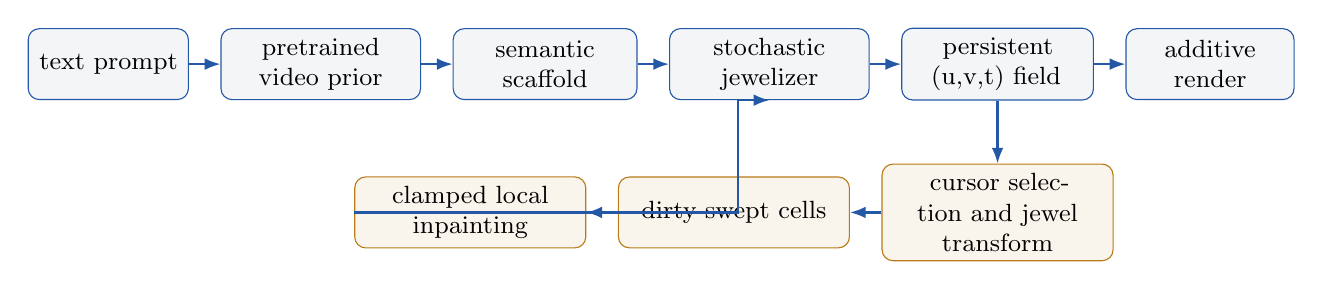
\begin{tikzpicture}[
  node distance=5mm and 4mm,
  box/.style={draw=jewelblue,rounded corners,fill=softgray,align=center,minimum height=9mm,text width=27mm,font=\small},
  action/.style={draw=jewelgold,rounded corners,fill=jewelgold!8,align=center,minimum height=9mm,text width=27mm,font=\small},
  arr/.style={-{Latex[length=2mm]},thick,jewelblue}
]
\node[box,text width=18mm] (text) {text prompt};
\node[box,text width=23mm,right=of text] (prior) {pretrained video prior};
\node[box,text width=21mm,right=of prior] (scaffold) {semantic scaffold};
\node[box,text width=23mm,right=of scaffold] (jewelizer) {stochastic jewelizer};
\node[box,text width=22mm,right=of jewelizer] (field) {persistent \uvt{} field};
\node[box,text width=19mm,right=of field] (video) {additive render};
\draw[arr] (text) -- (prior);
\draw[arr] (prior) -- (scaffold);
\draw[arr] (scaffold) -- (jewelizer);
\draw[arr] (jewelizer) -- (field);
\draw[arr] (field) -- (video);

\node[action,below=8mm of field] (drag) {cursor selection and jewel transform};
\node[action,left=of drag] (mask) {dirty swept cells};
\node[action,left=of mask] (repair) {clamped local inpainting};
\draw[arr] (field) -- (drag);
\draw[arr] (drag) -- (mask);
\draw[arr] (mask) -- (repair);
\draw[arr] (repair.west) -| ([xshift=-4mm]jewelizer.south) -- (jewelizer.south);
\end{tikzpicture}
\caption{Revised target system. A pretrained raster video prior supplies global semantics; the
jewelizer emits the persistent explicit state. Editing moves protected primitives, marks source,
destination, and swept cells dirty, and resamples only those cells while the rest remains exact.}
\label{fig:system}
\end{figure}

\section{Relationship to Prior Work and Claim Scope}

Modern Gaussian splatting was popularized for explicit 3D radiance fields by Kerbl et
al.~\cite{kerbl2023gaussians}. Dynamic-view methods subsequently added deformation, time, or native
higher-dimensional primitives~\cite{wu2024four,li2024spacetime}. Those systems reconstruct a
view-dependent 3D scene; our target is the displayed 2D RGB video itself, without recovering
physical depth or novel views.

That narrower video-representation lane is also established. Splatter a Video embeds monocular
video into canonical 3D Gaussians with motion~\cite{sun2024splatter}. VeGaS uses folded Gaussian
distributions to obtain time-conditioned 2D Gaussians and supports editing~\cite{smolak2024vegas}.
GSVC predicts frame-level 2D Gaussian sets from previous frames for compression~\cite{wang2025gsvc}.
GaussianVideo learns time-varying deformations of 2D Gaussians~\cite{lee2025gaussianvideo}.
Most directly, GaRV encodes videos as 3D Gaussians in a space-time volume~\cite{shah2026garv}.
HyperGS amortizes reconstruction by predicting per-frame Gaussian representations feed-forward from
input video~\cite{zohra2026hypergs}. Therefore, \textbf{we do not claim to be first to reconstruct
2D video with Gaussian splats, nor first to use a Gaussian space-time volume.}

Generative Gaussian work is substantial but usually targets 3D objects, rooms, or dynamic 3D
scenes. GaussianCube and L3DG learn structured or latent generative models of 3D
Gaussians~\cite{zhang2024gaussiancube,roessle2024l3dg}. VideoRFSplat generates text-conditioned 3D
scenes with a video model~\cite{go2025videorfsplat}; Diff4Splat predicts a deformable 3D Gaussian
scene from an image, camera path, and optional text~\cite{pan2026diff4splat}. DiffSplat repurposes a
large image diffusion prior to generate Gaussian splat grids and reports a rendering loss as
important for coherence across novel views~\cite{lin2025diffsplat}. This supports inheriting mature
raster priors and supervising rendered output rather than treating independent Gaussian-parameter
losses as a complete appearance objective.

The jewel births are also a marked spatiotemporal point set. Point Set Diffusion directly models
conditional spatial and spatiotemporal point processes without an intensity-function
factorization~\cite{ludke2024pointset}, while point-cloud flow work emphasizes that permutation
invariance and the coupling between noise and unordered targets materially affect the learned
transport~\cite{hui2025notsoptimal}. These results motivate a stochastic set objective; they do not
remove the need for a coherent video-level condition in the present task.

Our provisional distinction is the combination of: (1) direct generation of the displayed 2D
video as an anisotropic \uvt{} Gaussian field, (2) persistent stable-ID carry and birth emission
across overlapping time windows, and (3) hard-local jewel manipulation followed by constrained
latent repair. Our August 2026 search found no published system with this exact combination.
However, absence from a search is not proof of priority, and the current project has not yet shown
generalizing text-to-video generation. We therefore use ``toward'' in the title and reserve any
first-of-kind claim for a completed, externally benchmarked model and a broader review.

\begin{table}[H]
\centering
\footnotesize
\caption{Positioning against the closest video-Gaussian families. ``Amortized'' means a shared
encoder predicts a representation from input video; it is not the same as unconditional or
text-conditioned generation from noise.}
\label{tab:related}
\begin{tabularx}{\linewidth}{@{}lXXXX@{}}
\toprule
Method & Native target & Temporal form & Shared prediction & Primary goal \\
\midrule
VeGaS & 2D video & folded 3D Gaussians, conditional slices & no & representation/editing \\
GSVC & 2D video & linked per-frame 2D splats & no & compression \\
GaussianVideo & 2D video & time-deformed 2D splats & no & representation; codec \\
GaRV & 2D video & 3D space-time Gaussians & encoder/decoder scheme & random-access decoding \\
HyperGS & 2D video & predicted per-frame 2D splats & yes, from video & amortized encoding \\
\jewels{} (target) & 2D video & persistent anisotropic \uvt{} field & from noise and text & generation/editing \\
\bottomrule
\end{tabularx}
\end{table}

\section{Method}

\subsection{Video as an additive space-time field}

Let the normalized video domain be $\Omega=[-1,1]^3$, with a query
$\mathbf{x}=(u,v,t)\in\Omega$. Jewel $i$ has center $\boldsymbol\mu_i\in\R^3$, symmetric positive
definite covariance $\boldsymbol\Sigma_i\in\R^{3\times3}$, weight logit $\ell_i$, base color
$\mathbf{c}_i\in\R^3$, and a first-order color matrix
$\mathbf{G}_i\in\R^{3\times3}$. Its contribution is
\begin{align}
q_i(\mathbf{x}) &= (\mathbf{x}-\boldsymbol\mu_i)^\top
\boldsymbol\Sigma_i^{-1}(\mathbf{x}-\boldsymbol\mu_i),\\
a_i(\mathbf{x}) &= \sigma(\ell_i)\exp[-q_i(\mathbf{x})/2],\\
\widehat{\mathbf{I}}(\mathbf{x}) &= \mathbf{b}+\sum_i a_i(\mathbf{x})
\left[\mathbf{c}_i+\mathbf{G}_i(\mathbf{x}-\boldsymbol\mu_i)\right],
\label{eq:renderer}
\end{align}
where $\mathbf{b}$ is a learned constant background. This is additive accumulation, not ordered
alpha compositing. The P1 color term avoids requiring many constant-color primitives to approximate
smooth gradients.

Writing $\boldsymbol\Sigma_i=\mathbf{R}_i\operatorname{diag}(\mathbf{s}_i^2)\mathbf{R}_i^\top$
makes the motion interpretation explicit. If a principal axis of $\mathbf{R}_i$ tilts into time,
the support is a sheared tube through the volume. Rendering a frame means querying the plane at its
$t$ coordinate. The representation therefore has continuous random access in space and time.

Training samples arbitrary voxels, minimizes RGB MSE, and periodically splits high-gradient
primitives while pruning low-weight ones. Euclidean-center kNN supplies candidate splats; exact
Mahalanobis weights are then evaluated for those candidates. Distance work is chunked to at most
100M point-center pairs, allowing 45k--120k-field experiments on an 8 GB RTX 2070 Super. Atomic
checkpoints include optimizer and random-generator state, giving exact continuation across process
failure and CPU/CUDA densification boundaries.

\subsection{Gauge-free features and deterministic tokenization}

Raw scale/quaternion parameters are unsuitable learning targets: quaternions double-cover rotation
and covariance axes may permute. We instead use the unique log-Euclidean coordinate
\begin{equation}
\log\boldsymbol\Sigma_i=\mathbf{R}_i\operatorname{diag}(2\log\mathbf{s}_i)\mathbf{R}_i^\top.
\end{equation}
The upper triangle contributes six values to a 22-D feature:
$[\boldsymbol\mu,\operatorname{triu}(\log\boldsymbol\Sigma),\mathbf{c},
\operatorname{vec}(\mathbf{G}),\ell]$. Decoding by eigendecomposition reconstructs a render-equivalent
field with approximately $10^{-6}$ maximum feature round-trip error.

Dense fields are packed into a fixed $32^3$ cell raster. The count-aware local encoder pools means,
variances, counts, occupancy, and canonical rank features; the sparse decoder emits only the
predicted variable number of jewels rather than allocating worst-case slots for every cell. A
train-only PCA over non-overlapping $2^3$ blocks maps eight $24$-D fine cells into one $96$-D coarse
code. The resulting $16^3$ grid is modeled with rotating axial attention: one block attends along
$u$, the next $v$, and the next $t$. Three blocks communicate globally without materializing a
$4096^2$ attention matrix.

The full-field prior uses rectified flow~\cite{lipman2023flow}. For clean target latent $z_1$, noise
$z_0$, and interpolation $z_s=(1-s)z_0+sz_1$, the model regresses the velocity $z_1-z_0$ while
receiving time and an optional CLIP condition~\cite{radford2021clip}. Classifier-free dropout is
required before the null branch is interpreted.

\subsection{Persistent continuation}

Long video is not generated by concatenating independent fixed clips. A stride retains jewels whose
finite support intersects the overlap and copies their stable IDs and parameters exactly. The model
predicts only new birth counts and 22-D birth marks in frontier-local coordinates. A
$16\times16\times8$ raster of prefix counts and moments supplies spatially aligned context tokens.
This factorization turns ``splat density per unit time'' into an explicit birth process: the field
maintains a target contributor density while old jewels persist and new regions receive births.

\subsection{Scaffold-conditioned birth topology}

The first autonomous topology head receives two aligned
$16\times16\times8$ fields. The scaffold field is trilinearly pooled RGB from the next 16 video
frames. The carry field contains log density, occupancy, and mean opacity of jewels copied across
the frontier. A 3D convolutional encoder with global pooled context predicts one occupancy logit
$a_j$ and one positive-count value $q_j=1+\operatorname{softplus}(r_j)$ for every cell $j$. Its
continuous expected count is
\begin{equation}
\hat n_j=\sigma(a_j)q_j.
\end{equation}
Training combines balanced occupied/empty binary cross-entropy, Smooth-L1 error on
$\log(1+q_j)$ in positive cells, total log-count error, and an $L_1$ error between normalized count
distributions. The occupancy threshold is selected only on training fields by slot F1. Decoding
rounds positive counts and expands each cell into nested ranks $0,\ldots,\hat n_j-1$.

Topology uses a 1,024-rank contract because one initial UCF cell contains 919 births. The frozen
continuation mark flow uses 512 ranks, so coupling validates every predicted continuation cell
against that smaller capacity and raises an error rather than clipping. Carried features condition
the topology head but are never transformed; generated marks are appended after the exact carry.

\subsection{Stochastic mark realization and semantic guidance}

The first prompt-conditioned continuation baseline predicts a sparse count raster and one canonical
22-D mark per occupied cell/rank using deterministic Smooth-L1 regression. Canonical rank provides
a reproducible address, but it does not make the conditional output unimodal: several plausible
future actors, poses, and foreground colors can share the same local prefix and prompt. A paired
deterministic loss can therefore average mutually incompatible marks.

The controlled replacement holds target cells, counts, ranks, and carried jewels fixed and learns a
rectified flow over only the marks. For data mark \(y_1\), Gaussian noise \(y_0\), and
\(y_s=(1-s)y_0+sy_1\), the network predicts \(y_1-y_0\) while receiving the aligned prefix raster,
cell/rank address, flow time, and text. A hard projection maps sampled centers and finite-support
birth starts back to their declared cells without moving valid exterior edge-cell centers.

An oracle-guide variant additionally cell-pools the true future stride rendered at
\(24\times40\). It tests whether a coherent video scaffold contains the missing information needed
to realize jewels. Because that guide contains the answer at low resolution, it measures an
architectural ceiling and cannot be interpreted as text-to-video inference.

The first multiscale control constructs three guide volumes: the available future video and
low-pass versions at scales (2) and (4). A \(2\times2\times2\) subgrid in every birth cell
produces 24 local tokens, each containing RGB, horizontal/vertical/temporal RGB differences, local
coordinates, and scale identity. A cell/rank/noisy-mark query cross-attends only to tokens in its
addressed cell. For intermediate flow state \(y_s\) and predicted velocity \(v_\theta\), the
denoised endpoint
\begin{equation}
\hat y_1 = y_s + (1-s)v_\theta(y_s,s,c)
\end{equation}
is projected to the fixed topology and rendered on contiguous space-time patches. The tested
visual objective combines RGB MSE, spatial/temporal edge L1, opponent-chroma L1, and patch SSIM
while retaining feature-space flow loss for covariance stability. A follow-up hybrid keeps the
entire cell-RGB 3D-convolution/global guide path and adds local tokens only as residual evidence.

\subsection{Cursor edits and constrained repair}

A cursor selects jewel centers or support intersections in the parallelepiped. Translating a group
creates protected moved jewels and a dirty mask covering the source, destination, swept axis-aligned
bounding box, and a cell halo. Let $m\in\{0,1\}^{K}$ mark dirty latent cells and $z^{\rm clean}$ be
the original hierarchy. After each Euler flow step, sampling reclamps
\begin{equation}
z_{k+1}\leftarrow (1-m)\odot z^{\rm clean}+m\odot
\left[z_k+\Delta s\,v_\theta(z_k,s_k,c,m)\right].
\label{eq:clamp}
\end{equation}
The final merge contains untouched jewels, generated jewels decoded from dirty cells, and protected
moved jewels. This guarantees locality mechanically; visual reconciliation at the destination must
still be learned from edit tuples.

\section{Experimental Protocol}

Experiments use three tiers. A synthetic moving tube falsifies the basic motion representation.
CUHK Avenue~\cite{lu2013avenue} supplies fixed-camera fitting and generation-mechanics experiments.
UCF-101~\cite{soomro2012ucf101} supplies diverse action and appearance tests. Unless stated
otherwise, the short side is 160 pixels. The current prompt corpus uses 96-frame, 120k-jewel
joint fits with temporal-preserving spatial splitting.

We intentionally distinguish metrics. Fit-training PSNR is often computed on sampled voxels and is
not a publication-grade codec metric. ``Full-volume PSNR'' replays the complete saved field against
the decoded source. Tokenizer PSNR compares continuous samples rendered from the fitted target and
the decoded target, not decoded output against the source pixels. Energy distance evaluates latent
sample distributions. Correct/shuffled/null continuation controls use identical targets and model
weights. These quantities answer feasibility questions and should not be compared directly with
published rate-distortion or FVD results.

\section{Results and Discoveries}

\subsection{Reconstruction is viable, but not novel by itself}

The synthetic anisotropic-tube test reaches about \SI{55}{dB}. A real fixed-camera clip reaches
\SI{43.2}{dB} with 10k primitives; four recent UCF prompt-corpus fields reach 30.32--33.67 dB on
exact checkpoint replay. Figure~\ref{fig:promptfit} shows the source, 120k-jewel reconstruction, and
five-times-amplified absolute error for basketball. Class identity, player silhouettes, court
geometry, and dominant colors survive. Error concentrates on thin limbs, the ball, faces, object
edges, and motion boundaries.

\begin{figure}[H]
\centering
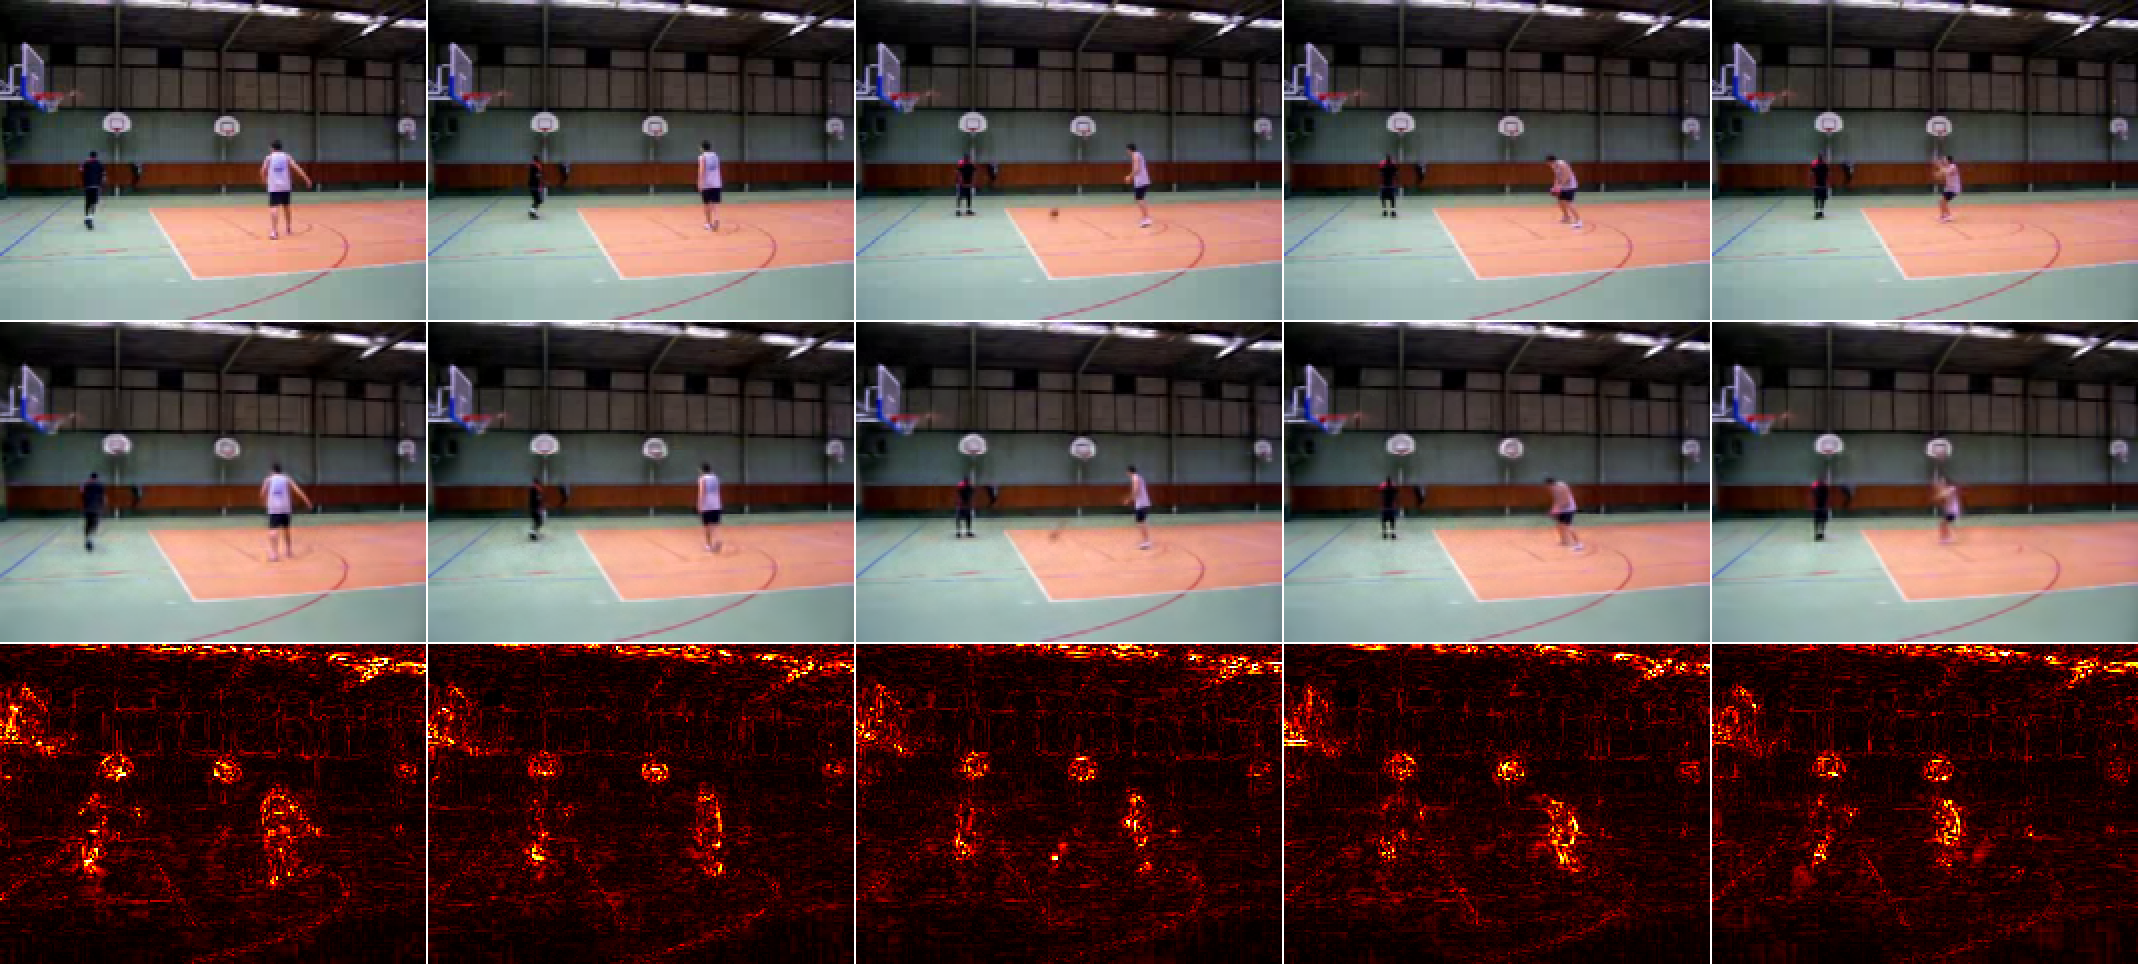
\includegraphics[width=0.90\linewidth]{../sol/results/prompt_smoke/previews_shard0/v_Basketball_g01_c03_w000000/contact_sheet.png}
\caption{Exact 96-frame checkpoint replay sampled at frames 0, 24, 48, 72, and 95. Rows are source,
120k-jewel reconstruction, and $5\times$ mean absolute RGB error. Full replay PSNR is
\SI{33.67}{dB}.}
\label{fig:promptfit}
\end{figure}

The covariance is not an ornamental parameter. Median anisotropy is about 2.8--3.3 on real footage,
versus about 1.2 on the synthetic background-dominated test. More importantly, attempts to impose a
soft Voronoi partition reduced both reconstruction and cross-seed canonicality. On one real clip,
additive splats score \SI{43.2}{dB} with a 0.621 normalized cross-seed Chamfer ratio; vanilla
Voronoi scores \SI{36.8}{dB}/0.745. A background pseudo-cell recovers some PSNR but not canonicality;
Lloyd relaxation collapses to \SI{33.0}{dB}/0.784. Equalizing cell sizes fights the desired
content-adaptive allocation, so the branch was removed.

\subsection{Useful density is a rate, not a raw count}

At 45k total jewels, temporal $3\sigma$ support intersects roughly 6.2k splats per Avenue frame, but
only 3.9k exceed 5\% potential peak alpha and the opacity-weighted effective count is 3.3k. UCF is
lower: 3.6k and 2.9k. Thus a nominally dense field remains below the desired 5k--10k effective
contributors per frame.

The naive 90k isotropic control demonstrates why. It nearly doubles observed births per frame,
shortens median support from 5 to 3 frames, increases effective contributors only 30.3\%, and lowers
PSNR. Figure~\ref{fig:density} shows that extra count does not recover more useful detail.

\begin{table}[H]
\centering
\small
\caption{Matched UCF density control. The successful next control preserves temporal extent and
splits spatial axes rather than shrinking every axis.}
\label{tab:density}
\begin{tabular}{@{}lrrr@{}}
\toprule
Measurement & 45k isotropic & 90k isotropic & Change \\
\midrule
Peak alpha $\geq5\%$/frame & 3,595 & 4,724 & +31.4\% \\
Effective contributors/frame & 2,933 & 3,822 & +30.3\% \\
Full-volume PSNR & 34.136 & 33.062 & $-1.074$ dB \\
Mean support lifespan (frames) & 8.41 & 5.58 & $-33.6\%$ \\
Median support lifespan (frames) & 5 & 3 & $-40.0\%$ \\
Observed births/frame & 659 & 1,290 & +95.6\% \\
Fit runtime (minutes) & 56.8 & 79.7 & +40.3\% \\
\bottomrule
\end{tabular}
\end{table}

\begin{figure}[H]
\centering
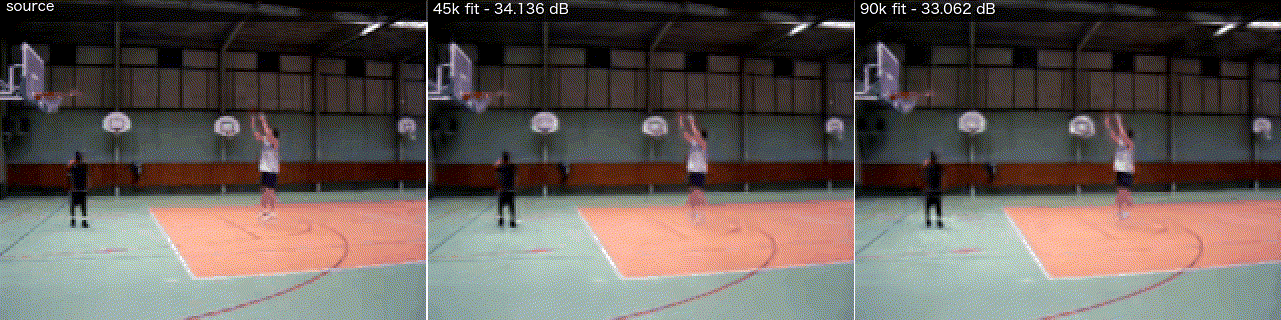
\includegraphics[width=\linewidth]{../sol/results/ucf_90k_density/source_45k_90k_frame32.png}
\caption{Source, 45k fit, and 90k isotropic fit at the same UCF frame. Doubling count increases
short-lived fragments rather than useful detail and reduces full-volume PSNR.}
\label{fig:density}
\end{figure}

\subsection{A generative field prior works before it works well}

An early permutation-invariant SetDiT flow model directly generated 6,471-jewel Avenue fields from
noise. Scaling 5.8M, 58M, and 173M-parameter models under a frozen protocol monotonically improves
CLIP-Frechet distance from 0.31 to 0.20 to 0.16 and training loss from 1.148 to 1.066 to 0.993
(Figures~\ref{fig:scaling-quant} and~\ref{fig:scaling-qual}). Samples preserve scene layout,
palette, chirality flips induced by
mirror augmentation, and temporal stability, but fine pedestrians remain distorted. The flattening
curve identified data and representation density, rather than further model scaling on 231 windows,
as the next axis.

\begin{figure}[H]
\centering
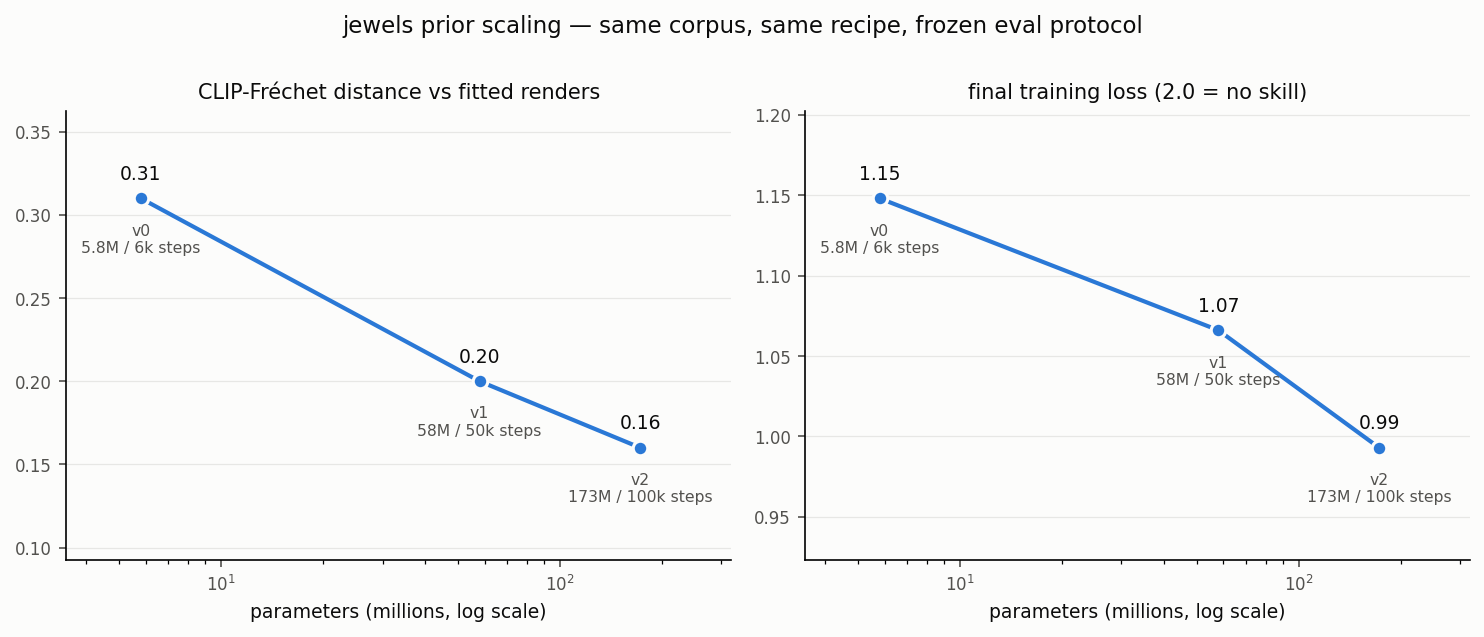
\includegraphics[width=0.86\linewidth]{../assets/scaling_curve.png}
\caption{Frozen scaling protocol for the first direct field prior. Improvement is monotone but
saturates on the small, single-scene corpus.}
\label{fig:scaling-quant}
\end{figure}

\begin{figure}[H]
\centering
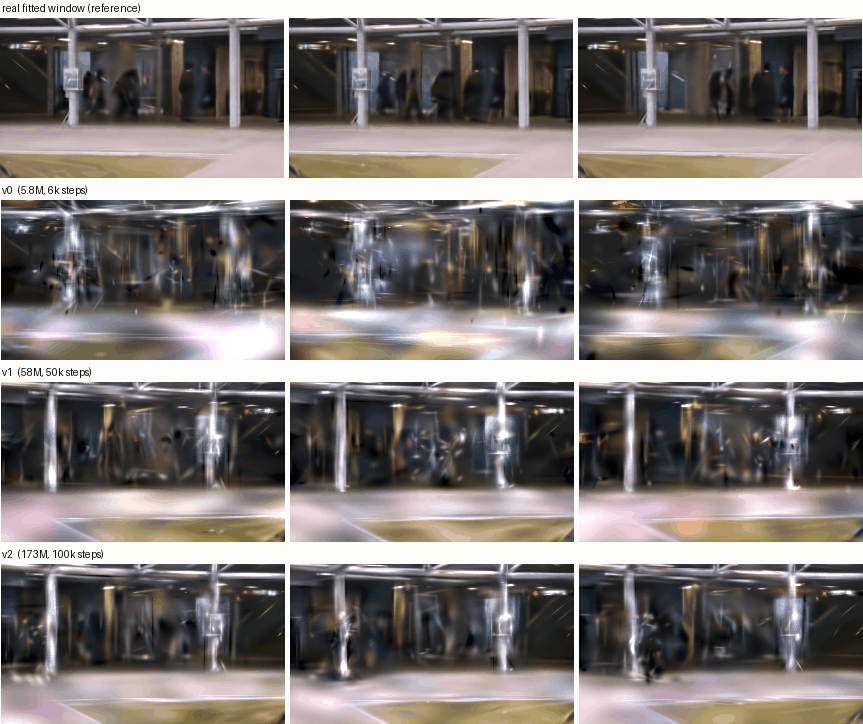
\includegraphics[width=0.78\linewidth]{../assets/v012_triptych.png}
\caption{A fitted reference and samples from v0, v1, and v2 at three times. Larger models preserve
the coarse scene more consistently, while people remain visibly under-resolved.}
\label{fig:scaling-qual}
\end{figure}

\subsection{Locality is load-bearing for the tokenizer}

On 121 dense Avenue windows, coarse cell pooling repeatedly achieved plausible aggregate PSNR while
erasing people. The first source-held-out tokenizer to preserve recognizable pedestrian silhouettes
uses a $32^3$ grid, 24 values per cell, near-one-jewel average locality, and canonical-rank-aware
decoding. Its 35-window audit reaches \SI{19.987}{dB} and 99.14\% count recovery. This remains a
weak 1.26$\times$ numeric bottleneck. The $2^3$ PCA hierarchy reduces 32,768 tokens to 4,096 and
loses only \SI{0.224}{dB}, making axial generation tractable.

Appearance is not solved. A bright red coat in held-out footage retains its figure but decodes tan.
Rare foreground chroma is overwhelmed by uniformly weighted 22-D jewel losses and sparse uniform
render samples. This is a regression-to-palette failure, not a channel-order bug. Foreground chroma
and perceptual metrics must accompany aggregate RGB PSNR.

Cross-domain controls sharpen the conclusion. Frozen Avenue weights reach only
\SI{17.786}{dB}/86.06\% count on UCF basketball; the identical architecture trained on that UCF
window reaches \SI{22.316}{dB}/97.13\%. Equal-exposure joint training reaches
\SI{20.278}{dB} on held-out Avenue and \SI{22.275}{dB} on UCF. The bottleneck can represent both,
but absolute cell/domain specialization remains substantial.

\begin{table}[H]
\centering
\small
\caption{Selected tokenizer and hierarchy results. PSNR compares fitted target and tokenizer
round-trip renders at fixed continuous samples.}
\label{tab:tokenizer}
\begin{tabularx}{\linewidth}{@{}XrrX@{}}
\toprule
Representation & Tokens & PSNR & Visual result \\
\midrule
$12\times12\times6$, 128-D & 864 & 18.940 & people erased \\
$16\times16\times8$, rank-v2 & 2,048 & 20.428 & people erased \\
$24\times24\times16$, pooled & 9,216 & 19.730 & faint traces \\
$32^3$, rank-aware, 24-D & 32,768 & \textbf{19.987} & people recognizable \\
$16^3$, PCA, 96-D & 4,096 & 19.763 & people retained \\
\bottomrule
\end{tabularx}
\end{table}

\subsection{Generation, continuation, and editing separate into distinct gates}

The 1.94M-parameter axial prior learns the coarse latent distribution: energy distance 0.2493 beats
CLIP nearest-neighbor retrieval (0.3164) and repeated scene mean (0.8473). Yet correct CLIP
conditioning is slightly worse than shuffled or unconditional conditioning (gain $-0.00171$).
With only four training cameras and one image embedding per window, the model learns scene-family
statistics, not semantic control.

Continuation gives a stronger causal control. Replacing one global prefix vector with aligned
$16\times16\times8$ local tokens produces the results in Table~\ref{tab:continuation} and
Figure~\ref{fig:continuation}. Correct context reduces standardized birth-feature MSE by 62.7\%
against disjoint shuffled context and recovers 99.95\% of births. Carried jewels are copied with
zero error. This is still an overfit to four views of one clip, but it proves that spatial
correspondence, not merely window identity, is required.

\begin{table}[H]
\centering
\small
\caption{Matched cell-local continuation control.}
\label{tab:continuation}
\begin{tabular}{@{}lrrr@{}}
\toprule
Metric & Correct & Shuffled & Null \\
\midrule
Birth-feature MSE & \textbf{0.4475} & 1.1988 & 2.1695 \\
Birth-count MAE/cell & \textbf{0.3310} & 3.7167 & 6.4994 \\
Future-field PSNR & \textbf{19.870} & 7.302 & $-29.735$ \\
\bottomrule
\end{tabular}
\end{table}

\begin{figure}[H]
\centering
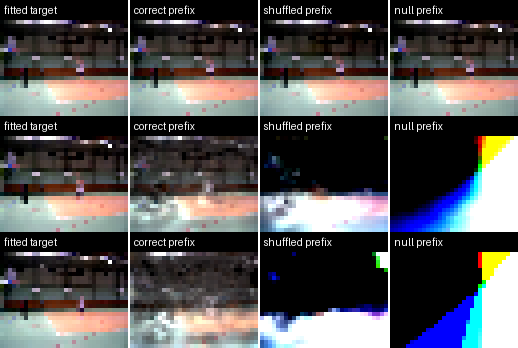
\includegraphics[width=0.75\linewidth]{../sol/results/streaming_continuation_local/continuation_controls_contact.png}
\caption{Start, middle, and end diagnostics for fitted target, correct prefix, disjoint shuffled
prefix, and null prefix. The extreme null output is not a video baseline because this overfit was
not trained with context dropout.}
\label{fig:continuation}
\end{figure}

The editor translates 281 real fitted jewels, dirties 448 of 4,096 coarse cells (10.94\%), and
merges 45,244 final jewels. Every clean coarse and fine latent is bit-identical. The repaired strip,
however, is visibly washed out. A mask-aware 5,000-step branch improves dirty latent MSE only from
1.8894 to 1.8848 and does not improve the visual. The result validates the editor invariant while
falsifying the current repair learner.

\subsection{Text preflight passes; direct deterministic generation washes out}

The prompt smoke test selects Basketball, HorseRiding, PlayingGuitar, and ApplyEyeMakeup from four
disjoint UCF source groups: 12 training videos and four group-held-out validation videos. Three
training phrasings and one unseen evaluation phrasing per class are embedded with frozen OpenCLIP
ViT-B/32. Each unseen phrase retrieves the correct training-phrase centroid; the minimum correct
versus best-wrong cosine margin is 0.2395 (Table~\ref{tab:prompt}).

\begin{table}[H]
\centering
\small
\caption{Held-out text geometry before jewel-model training.}
\label{tab:prompt}
\begin{tabular}{@{}lrrr@{}}
\toprule
Class & Correct cosine & Best wrong & Margin \\
\midrule
Basketball & 0.8641 & 0.5881 & 0.2760 \\
HorseRiding & 0.9004 & 0.6610 & 0.2395 \\
PlayingGuitar & 0.9037 & 0.6546 & 0.2490 \\
ApplyEyeMakeup & 0.9102 & 0.6229 & 0.2873 \\
\bottomrule
\end{tabular}
\end{table}

All 16 dense 120k-jewel fits are complete. A 0.84M-parameter direct continuation model is trained on
the 12 group-1--3 videos and evaluated on all four group-4 sources. With the prefix removed, the
correct unseen text template has mark MSE 1.1579 versus 1.1794 for shuffled action text and changes
free decoded counts by class. Thus prompt information reaches the model, but decoded videos remain
washed out and do not depict reliable action geometry.

The proposed immediate remedy was to split the sparse topology head into occupied-cell
classification and positive-count regression. We instead first held the entire target topology
fixed. Table~\ref{tab:washout} shows that oracle cells, counts, and ranks improve mean PSNR by only
\SI{0.172}{dB}. Predicted geometry and predicted color/gradient each independently collapse the
render, while predicted opacity is comparatively benign. Moreover, only 39.73\% of predicted
centers remain in their supplied spatial cell and 25.41\% in the full space-time birth cell. This is
a real contract defect, but it is not the main visual cause: even the oracle-topology render remains
washed out.

\begin{table}[H]
\centering
\small
\caption{Held-out deterministic washout decomposition averaged over four classes. ``Oracle
topology'' supplies target cells, counts, and ranks while predicting all 22-D marks. Other rows
replace only the named target mark group.}
\label{tab:washout}
\begin{tabularx}{\linewidth}{@{}XrX@{}}
\toprule
Output & Mean PSNR & Finding \\
\midrule
Free deterministic prediction & 14.060 dB & Topology and marks predicted \\
Predicted marks, oracle topology & 14.232 dB & Only +0.172 dB; still washed out \\
Predicted geometry only & 14.434 dB & Geometry error destroys structure \\
Predicted color/gradient only & 15.255 dB & Appearance regression independently washes out \\
Predicted opacity only & 24.816 dB & Opacity is not the dominant failure \\
\bottomrule
\end{tabularx}
\end{table}

\subsection{A stochastic jewelizer needs a coherent semantic scaffold}

A 1.54M-parameter mark flow trained for 12,000 steps with oracle topology restores edge energy but
not semantic coherence. Raw held-out samples average 15.064 dB and 84.4\% of target edge energy,
versus 14.232 dB and 59.8\% for deterministic marks, yet the GIFs show structured speckle rather
than recognizable action. Sampling avoids part of the conditional mean, but the local prefix and
four-class text vector do not determine global scene layout.

A second 12,000-step control adds the true future only as a \(24\times40\) guide. Table
\ref{tab:guide} and Figure~\ref{fig:guide} show the decisive result: the guided stochastic
jewelizer reaches 16.555 dB and 90.5\% edge energy, recovering the court/player, horse/rider,
guitar/player, and face/hand macro-layout. A corrected hard projection maps generated marks to the
declared topology while leaving every fitted target render-identical at 100 dB, so the gain is not a
projection artifact. Residual high-frequency noise remains substantial. Correct and shuffled text
are also similar under the oracle guide because the guide already supplies the future semantics.

\begin{table}[H]
\centering
\small
\caption{Held-out mark realization with target birth topology. Ratios are relative to the fitted
target render; the stochastic row is raw because the original projection was not target-preserving,
whereas the final guided row uses the corrected projection.}
\label{tab:guide}
\begin{tabular}{@{}lrrr@{}}
\toprule
Mark generator & Mean PSNR & Contrast ratio & Edge ratio \\
\midrule
Deterministic regression & 14.232 & 0.574 & 0.598 \\
Unguided stochastic flow & 15.064 & 0.775 & 0.844 \\
Oracle-video-guided flow & \textbf{16.555} & \textbf{0.856} & \textbf{0.905} \\
\bottomrule
\end{tabular}
\end{table}

\begin{figure}[H]
\centering
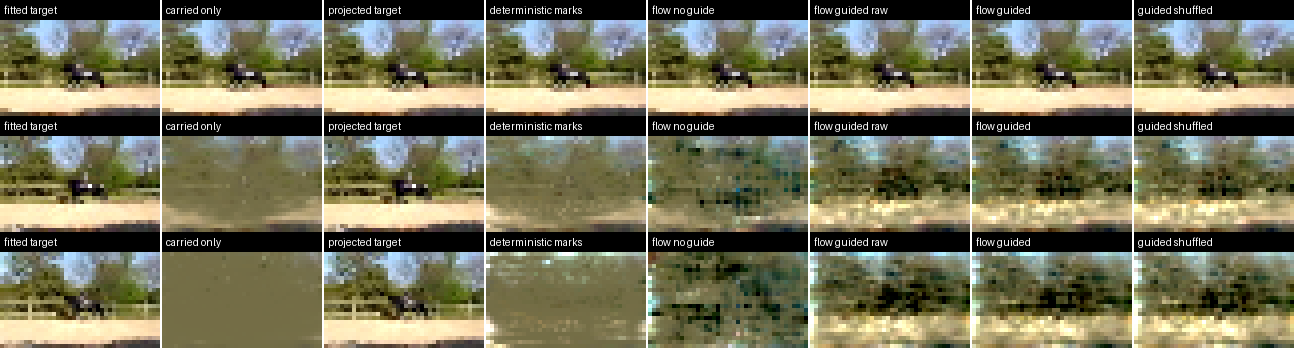
\includegraphics[width=\linewidth]{../sol/results/prompt_smoke/direct_prompted_streaming_3000/mark_flow_oracle_guide_12000/visual_contract_projection/HorseRiding_g04_mark_flow_controls_contact.png}
\caption{HorseRiding at three held-out future times. Columns compare the fitted target, carried
prefix alone, projection control, deterministic marks, zero-guide flow, guided raw and projected
flow, and shuffled text with the same oracle guide. The guide restores scene layout that topology
and stochasticity alone do not.}
\label{fig:guide}
\end{figure}

\subsection{Prompt scaffolds can be fitted at the intended contributor rate}

The official distilled LTX-2.3 pipeline generated a balanced set of 16 prompt videos: three
training phrasings and one unseen evaluation phrasing for each of the four action classes. All
16 complete at \(768\times512\), 49 frames, and 24 fps. Mean generation time is 172.98 seconds and
mean aggregate GPU peak is 9,399 MiB on the RTX 4090. Independent contact-sheet review preserves
the requested action and primary subject in every clip, so this corpus supplies substantially more
coherent prompt semantics than the direct jewel model.

Before fitting all generated videos, we scale the established 120k/96-frame budget by space-time
volume, which gives approximately 69k jewels, and round to a 72k ceiling. The first Basketball
evaluation-prompt fit takes 1,523.1 seconds and replays at \SI{28.182}{dB}. More importantly, its
opacity-weighted effective density averages 6,384 contributors/frame and ranges 5,485--7,626;
7,389/frame exceed 5\% potential peak alpha. Thus it lands inside the intended 5k--10k visual
regime rather than merely increasing raw total count.

The frozen contract then transfers cleanly across all four actions (Table~\ref{tab:ltxfits}). Mean
full-video PSNR is \SI{31.472}{dB}; mean effective density is 5,966 contributors/frame and mean
5\%-alpha count is 6,883/frame. PlayingGuitar is the instructive exception: its strict effective
count is 4,597/frame, slightly below the nominal floor, despite a strong reconstruction. Density is
therefore retained as a content-aware diagnostic rather than enforced as a blind scalar quota.
ApplyEyeMakeup reaches \SI{35.158}{dB} after a checkpoint-preserving 4090-to-2070S migration and
preserves face, hand, eye motion, and palette. Figure~\ref{fig:ltxfit} shows the weakest-PSNR
Basketball case: court, players, ball motion, and red uniforms survive, while fine fence/tree detail
and fast limbs remain soft. These pass as semantic-scaffold targets, not as final codec results.

\begin{table}[H]
\centering
\small
\caption{Frozen 49-frame/72k-jewel LTX reconstruction gate. Contributor counts are per-frame
means; ``effective'' is opacity weighted.}
\label{tab:ltxfits}
\begin{tabular}{@{}lrrr@{}}
\toprule
Class & PSNR (dB) & Effective & Above 5\% alpha \\
\midrule
Basketball & 28.182 & 6,384 & 7,389 \\
HorseRiding & 31.707 & 7,134 & 8,042 \\
PlayingGuitar & 30.839 & 4,597 & 5,339 \\
ApplyEyeMakeup & 35.158 & 5,749 & 6,762 \\
\midrule
Mean & 31.472 & 5,966 & 6,883 \\
\bottomrule
\end{tabular}
\end{table}

\begin{figure}[H]
\centering
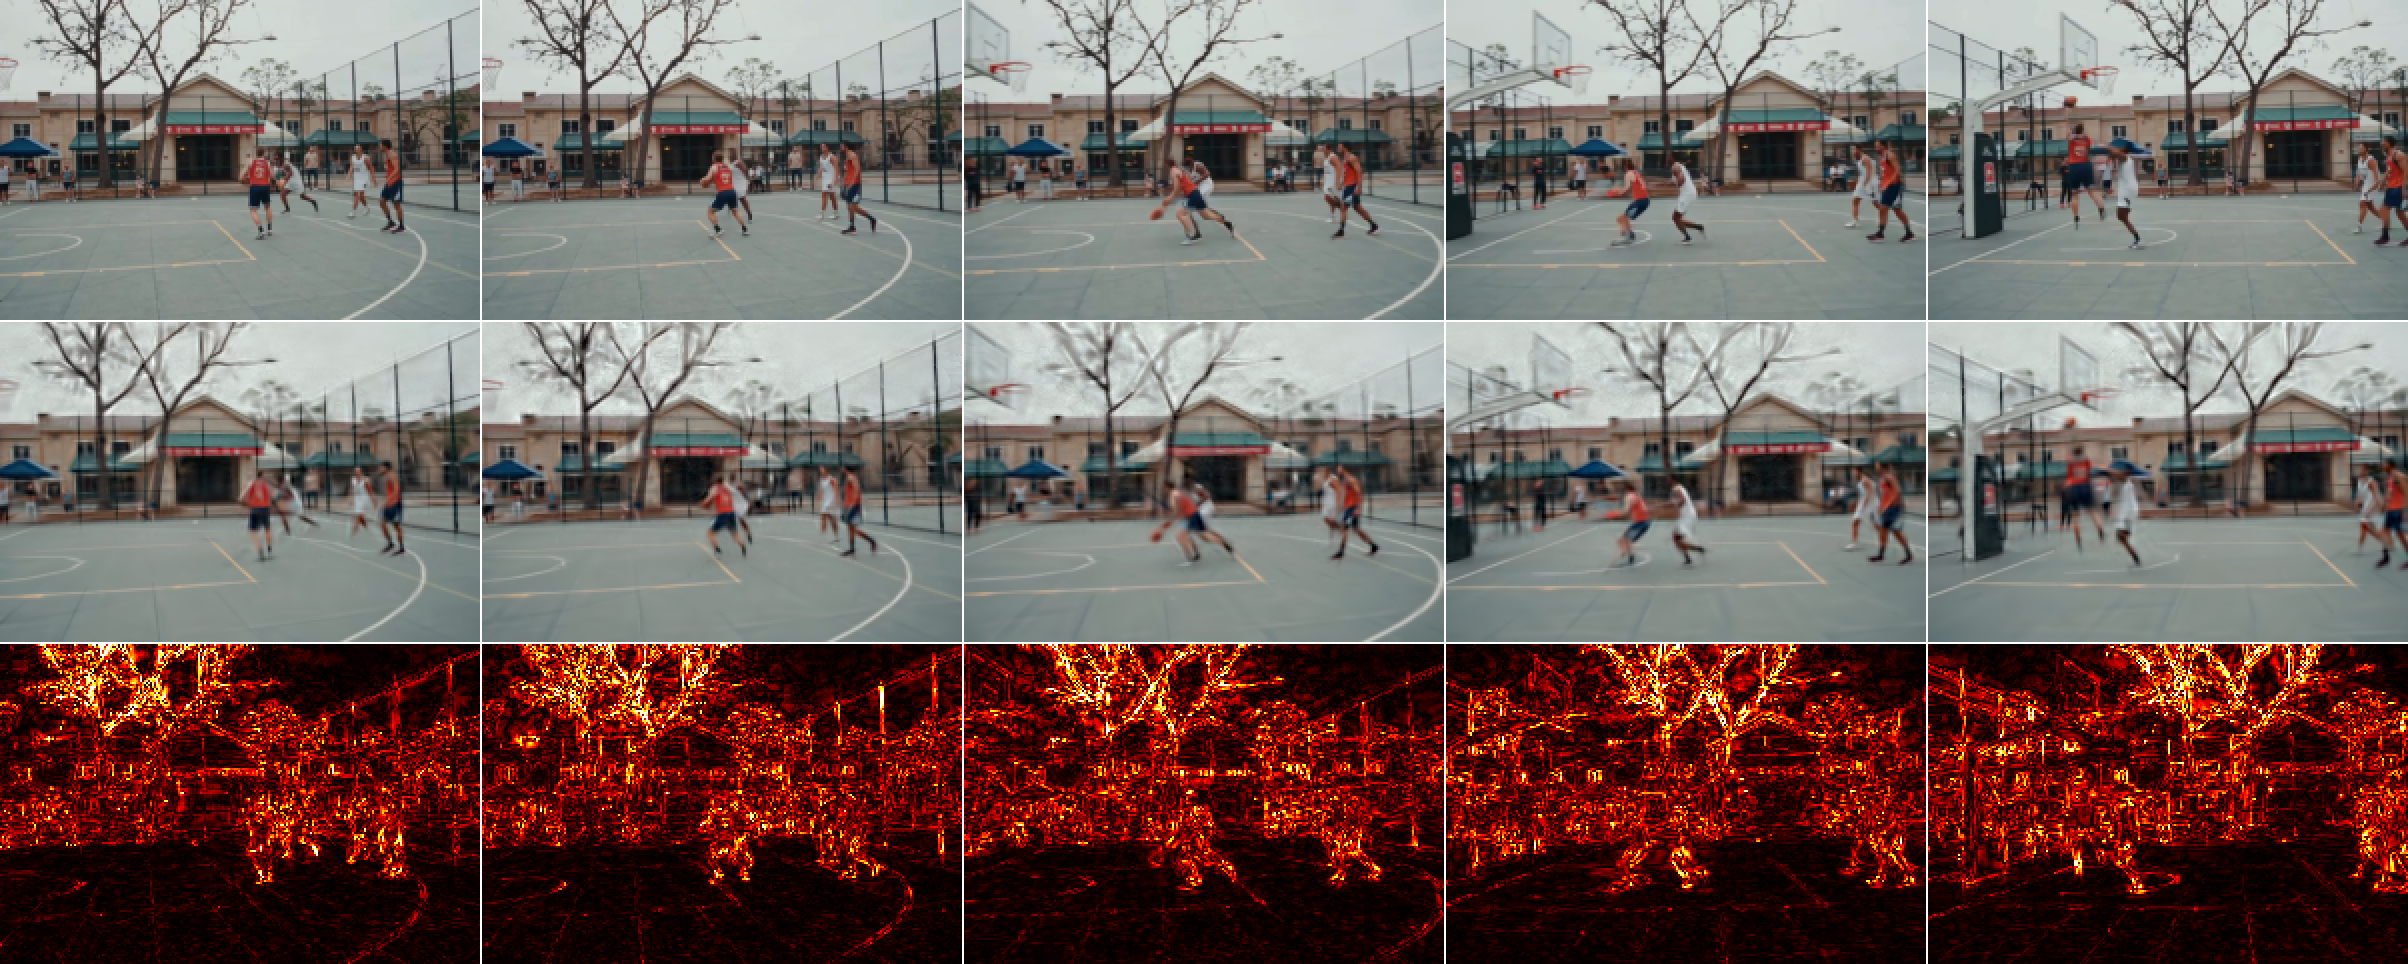
\includegraphics[width=\linewidth]{../sol/results/ltx_scaffold_v1/jewel_fit_gate_72k/contact_sheet.png}
\caption{LTX Basketball scaffold at frames 0, 12, 24, 36, and 48. Rows show decoded source,
72k-jewel reconstruction, and \(5\times\) absolute RGB error. Full replay PSNR is
\SI{28.182}{dB}; measured effective density is 6,384 jewels/frame.}
\label{fig:ltxfit}
\end{figure}

\subsection{Multiscale and render controls expose non-dominating trades}

Table~\ref{tab:multiscale} reports the token-only multiscale model with render weight 2 against the
cell-RGB v1 guide under identical topology, noise, sampling steps, held-out sources, and renderer.
It raises target-relative contrast and edge energy, but lowers paired PSNR, mean frame-global SSIM,
saturation, and temporal stability. Per-class behavior is inconsistent: ApplyEyeMakeup improves,
Basketball is nearly flat, HorseRiding loses SSIM, and PlayingGuitar loses \SI{0.948}{dB}. Visual
inspection likewise finds cleaner local regions but no reliable action-level improvement. The
branch therefore does not pass the realizer gate.

Two controls separate architecture from objective. Keeping the complete raster path and adding
tokens with feature loss alone lowers every aggregate appearance metric, reaching 16.240 dB and
0.8345 SSIM. Keeping only the v1 raster architecture and applying render weight 2 raises contrast
but loses 0.547 dB and 0.0087 SSIM. Reducing the predeclared weight to 0.5 improves mean SSIM by
0.0082, contrast ratio by 0.0795, and edge ratio by 0.0200, but loses 0.307 dB, reduces saturation,
and increases excess temporal change. ApplyEyeMakeup improves by 0.584 dB, whereas PlayingGuitar
loses 1.574 dB and overshoots both contrast and motion. The detail signal is real, but the present
uniform tiny-patch estimator is not stable across actions.

\begin{table}[H]
\centering
\small
\caption{Matched four-class guided mark realization. Ratios target 1.0; temporal change above 1.0
indicates excess flicker/motion energy.}
\label{tab:multiscale}
\begin{tabular}{@{}lrrrrrr@{}}
\toprule
Guide/objective & PSNR & SSIM & Contrast & Edge & Saturation & Temporal \\
\midrule
Raster, feature flow & \textbf{16.555} & 0.8475 & 0.8555 & 0.9050 & \textbf{0.9371} & \textbf{1.7236} \\
Tokens, feature+render (2.0) & 16.419 & 0.8441 & 0.8694 & 0.9108 & 0.9194 & 1.7833 \\
Raster+tokens, feature flow & 16.240 & 0.8345 & 0.8519 & 0.8925 & 0.9209 & 1.7250 \\
Raster, feature+render (2.0) & 16.009 & 0.8388 & 0.8936 & 0.9021 & 0.8836 & 1.7725 \\
Raster, feature+render (0.5) & 16.248 & \textbf{0.8557} & \textbf{0.9351} & \textbf{0.9251} & 0.9167 & 1.8055 \\
\bottomrule
\end{tabular}
\end{table}

The token-only model exchanged cross-cell macro context for within-cell detail, and the residual
token control shows that simply stacking both paths is not sufficient at this data scale. The
render controls likewise reject scalar-weight tuning as the fix: their local losses can sharpen
detail while amplifying motion inconsistently. We retain v1 for the cross-domain scaffold gate and
reserve future render supervision for foreground/motion-aware sampling with an explicit temporal
stability term.

\subsection{UCF-trained jewel realization transfers to unseen LTX scaffolds}

Before viewing any cross-domain output, we declare that v1 must beat deterministic UCF continuation
in macro PSNR and SSIM, move contrast and edge ratios toward 1.0, retain at least 98\% mean
birth-cell adherence, and preserve a recognizable primary subject/action in at least three of four
contact sheets. Training remains the original 12 UCF sources; validation replaces only the four
group-4 clips with unseen LTX evaluation-prompt scaffolds. The first 16-frame continuation view,
sampling noise, target topology, and renderer are matched across controls.

Table~\ref{tab:ltxtransfer} shows that the gate passes. Guided flow gains \SI{1.565}{dB} and 0.2782
SSIM over deterministic continuation. Contrast rises from 0.426 to 0.743, edge energy from 0.486 to
0.830, temporal change reaches 0.981 of target, and birth-cell adherence is 99.08\%. Every class
improves in PSNR and SSIM: PSNR gains span \SIrange{0.590}{2.627}{dB}. Projection without the video
guide is insufficient, reaching only \SI{12.810}{dB}; the semantic raster is the causal input.

\begin{table}[H]
\centering
\small
\caption{UCF-trained mark realization on four unseen LTX scaffolds. Appearance and temporal ratios
target 1.0; birth-cell values report projected adherence.}
\label{tab:ltxtransfer}
\begin{tabular}{@{}lrrrrrr@{}}
\toprule
Panel & PSNR & SSIM & Contrast & Edge & Temporal & Birth cell \\
\midrule
Deterministic continuation & 13.777 & 0.4160 & 0.4261 & 0.4860 & 0.7873 & 0.1021 \\
Flow, no guide & 12.810 & 0.3454 & 0.5048 & 0.6691 & 0.9583 & 0.9739 \\
Flow, LTX guide & \textbf{15.342} & 0.6942 & \textbf{0.7428} & \textbf{0.8300} & \textbf{0.9815} & \textbf{0.9908} \\
Flow, guide + shuffled text & 15.319 & \textbf{0.6955} & 0.7429 & 0.8260 & 0.9853 & 0.9904 \\
\bottomrule
\end{tabular}
\end{table}

\begin{figure}[H]
\centering
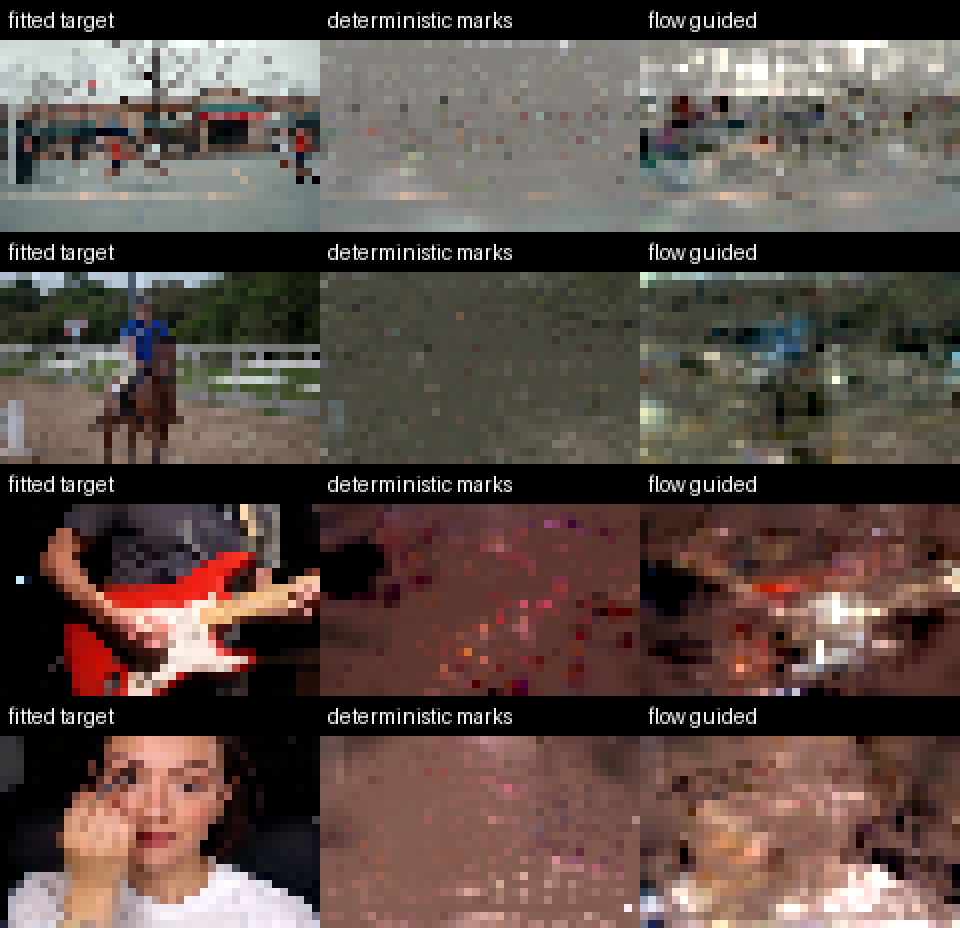
\includegraphics[width=0.68\linewidth]{../sol/results/ltx_scaffold_v1/realizer_eval/transfer_gate_contact.png}
\caption{One matched future time per LTX class. Columns show fitted target, deterministic UCF
continuation, and guided projected flow; rows are Basketball, HorseRiding, PlayingGuitar, and
ApplyEyeMakeup. Horse, guitar, and makeup retain recognizable primary subjects/actions. Basketball
retains court/player layout but remains the weakest and blurriest transfer.}
\label{fig:ltxtransfer}
\end{figure}

Correct and shuffled text are effectively tied under the true LTX guide: correct text changes PSNR
by only +0.023 dB and SSIM by -0.00134. Thus the jewel model has not learned independent prompt
semantics; those semantics arrive through the prompt-generated raster scaffold. This licenses the
next experiment: predict occupied cells, counts, and ranks from that scaffold while stable-ID
overlap state persists. Direct text-to-jewel distillation remains a later corpus-scale question.

\subsection{Learned scaffold topology matches the oracle continuation ceiling}

We train the 0.88M-parameter topology head for 3,000 updates on 72 complete initial and
continuation views from the 12 UCF fields, then evaluate without adaptation on 12 views from the
four LTX fits. The run takes 41.96 seconds on an RTX 2070 Super. Table~\ref{tab:topologyhead}
establishes causal scaffold use: the correct guide beats cross-class shuffled, null, and per-stride
train-mean controls in slot F1 and count correlation. Removing carry drops slot F1 to 0.5374 and
overpredicts births by 19.3\%, making persistent overlap a load-bearing input rather than a merge
detail.

\begin{table}[H]
\centering
\small
\caption{Held-out LTX topology over all initial and continuation views. Threshold calibration and
the train-mean count field use UCF training data only.}
\label{tab:topologyhead}
\begin{tabular}{@{}lrrr@{}}
\toprule
Topology input & Slot F1 & Count correlation & Birth ratio \\
\midrule
Correct scaffold + carry & \textbf{0.6636} & \textbf{0.6010} & 0.9390 \\
Cross-class scaffold + carry & 0.6092 & 0.4728 & 0.9341 \\
Null scaffold + carry & 0.6091 & 0.4628 & 0.8829 \\
Per-stride UCF train mean & 0.6222 & 0.3147 & 0.9378 \\
Correct scaffold, no carry & 0.5374 & 0.3440 & 1.1933 \\
\bottomrule
\end{tabular}
\end{table}

An oracle-mark rollout initially appeared to retain only 56--59\% of fitted effective density: it
discarded every predicted rank without an exact counterpart in one fitted decomposition. That is
not a valid generative density test because additive Gaussian decompositions are non-unique. Two
source-level cross-validation folds that add two LTX fits strengthen count discrimination but do
not materially change exact-rank retention, arguing against fitting a larger corpus solely to fix
that diagnostic.

The decisive experiment instead synthesizes every predicted rank with the frozen UCF mark flow.
It evaluates the only LTX continuation view supported by the flow's 32-frame prefix contract,
frames 32--48. The first 32 frames and carried jewels are fitted seed state; the learned topology
uses correct scaffold RGB and carry. For the shuffled control only the topology guide is rotated to
another class; the mark flow still sees the correct LTX guide and text. Thus any learned/shuffled
difference is attributable to the topology field.

Table~\ref{tab:autonomoustopology} shows that learned topology predicts 70,724 births versus 70,952
targets and all four class means lie between 5,598 and 6,449 effective contributors/frame. It loses
only 0.028 dB and 0.0030 SSIM to generated marks under oracle topology. Its largest cell has 113
ranks, below the frozen flow's 512-rank capacity; spatial adherence is 100\%, mean birth-cell
adherence exceeds 98.8\%, and carried features remain bit-identical with zero maximum error.

\begin{table}[H]
\centering
\small
\caption{Frozen mark realization on the held-out LTX 32--48 continuation. Appearance ratios target
1.0; density is opacity-weighted effective contributors/frame.}
\label{tab:autonomoustopology}
\begin{tabular}{@{}lrrrrr@{}}
\toprule
Panel & PSNR & SSIM & Contrast & Edge & Density \\
\midrule
Carried only & 13.529 & 0.3521 & 0.3263 & 0.3438 & 1,924 \\
Oracle topology, generated marks & 15.492 & 0.6997 & 0.7252 & 0.8197 & 6,252 \\
\textbf{Learned topology, generated marks} & \textbf{15.464} & \textbf{0.6967} & \textbf{0.7202} & \textbf{0.8250} & \textbf{5,822} \\
Shuffled topology, correct mark guide & 15.353 & 0.6927 & 0.7314 & 0.8170 & 5,781 \\
\bottomrule
\end{tabular}
\end{table}

\begin{figure}[H]
\centering
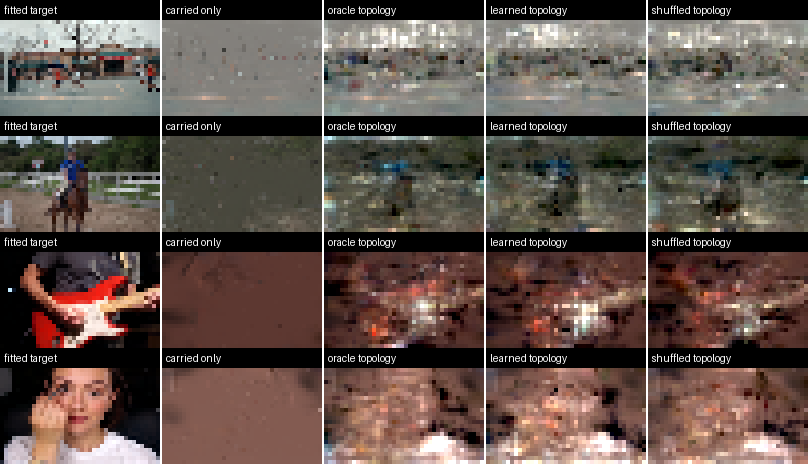
\includegraphics[width=0.88\linewidth]{../sol/results/ltx_scaffold_v1/topology_eval/autonomous_topology_contact.png}
\caption{One middle continuation frame per LTX class. Columns show fitted target, carried-only
state, generated marks with oracle topology, generated marks with learned topology, and generated
marks with cross-class-shuffled topology. Learned and oracle topology preserve the same macro-layout
and share the same motion-region noise, localizing that residual error in mark realization.}
\label{fig:autonomoustopology}
\end{figure}

This passes learned topology, intended density, and exact carry for one held-out continuation
stride. The learned/shuffled visual margin is modest because coarse occupancy is nearly dense and
the correct mark guide supplies strong semantics, although slot overlap and correlation remain
causally better. Initial jewel generation and two free-running generated-mark strides are still
required before the hybrid system is end-to-end.

\section{What Has Been Falsified}

Failures have been used as architectural evidence rather than hidden tuning history:

\begin{table}[H]
\centering
\small
\caption{Selected falsifications and the resulting decision.}
\label{tab:falsified}
\begin{tabularx}{\linewidth}{@{}XX@{}}
\toprule
Failed hypothesis & Decision \\
\midrule
Soft Voronoi improves canonicality & Removed; additive wins reconstruction and normalized cross-seed Chamfer. \\
More raw splats automatically increase useful density & Rejected; audit contributor rate and preserve temporal axes during split. \\
Aggregate PSNR selects a visually useful tokenizer & Rejected; require held-out motion silhouettes and foreground chroma checks. \\
Global prefix context is sufficient for births & Rejected; aligned cell-local context improves future-field PSNR by 3.41 dB. \\
The six-camera CLIP prior uses semantics & Rejected; correct condition does not beat shuffled/null. \\
Sparse count/topology error is the primary washout cause & Rejected; exact target topology adds only 0.172 dB. \\
Stochastic marks alone recover coherent video & Rejected; edge energy returns, but samples remain structured noise without a video guide. \\
Local multiscale tokens automatically improve the raster guide & Rejected; token-only and residual-hybrid controls both lose the matched visual gate. \\
Scalar render-loss tuning cures washout & Rejected; detail improves at weight 0.5, but one action becomes less faithful and less stable. \\
Exact fitted cell/rank overlap measures generated density & Rejected; synthesizing all predicted ranks restores 5,822 effective contributors/frame and oracle-level rendering. \\
Mask visibility alone teaches repair & Rejected; train explicit edit tuples with protected-jewel summaries. \\
Further model scaling solves the sparse prior & Deprioritized; the curve saturates on 231 single-scene windows. \\
\bottomrule
\end{tabularx}
\end{table}

\section{Limitations}

\begin{itemize}
  \item \textbf{No end-to-end autonomous text-to-jewel result.} The hybrid path now predicts
  continuation topology and marks from an LTX scaffold, but the first 32 jewel frames and carried
  prefix are still fitted seed state. The jewel model's correct and shuffled text controls remain
  tied because semantics live in the prompt-generated scaffold.
  \item \textbf{Small and specialized corpora.} The generative results use one fixed-camera scene;
  the continuation result is an overfit; the prompt corpus contains only 16 videos.
  \item \textbf{Fixed camera and no cuts.} Global camera motion shears most primitives at once and
  spends density on camera motion. Camera tokens or explicit stabilization are future work.
  \item \textbf{Low resolution.} Current fits use a 160-pixel short side. PSNR values are not
  comparable to full-resolution codec papers without a matched rate-distortion protocol.
  \item \textbf{Appearance loss.} Uniform feature and RGB losses underweight rare foreground color,
  faces, hands, and thin objects. The red-to-tan coat error is a concrete warning.
  \item \textbf{Single learned-topology stride.} Fitted cells and ranks are removed only for frames
  32--48. Initial topology exceeds the frozen flow's old 512-rank capacity in one observed UCF cell,
  and two generated-mark strides with model-produced carry have not yet been rendered.
  \item \textbf{Weak rendered topology selectivity.} Correct scaffold topology beats shuffled/null
  in count space, but shuffled-topology rendering is only 0.111 dB below correct because occupancy
  is nearly dense and the mark flow still sees the correct guide. Finer/adaptive density fields may
  be needed for topology itself to control semantics.
  \item \textbf{Motion-region mark noise.} Learned and oracle topology share blur/noise on moving
  actors, hands, and thin objects. This localizes the next visual error to mark realization rather
  than insufficient birth count.
  \item \textbf{Pure-PyTorch rendering.} Exact kNN/Mahalanobis evaluation is useful for research but
  slower than a tile CUDA rasterizer. Current reconstruction is optimization-based, not amortized.
  \item \textbf{Edit quality.} Clean-region identity is exact, but dirty-region synthesis is not yet
  visually useful and may create additive collisions with protected moved jewels.
  \item \textbf{Novelty is provisional.} Closely related literature is moving quickly. A formal
  claim requires a complete system, broader search, matched baselines, and external review.
\end{itemize}

\section{Why an Explicit Jewel Field Rather Than a Raster Latent?}

The relevant comparison is not ``jewels versus diffusion.'' A jewel field specifies the state that
is represented and rendered; diffusion, flow matching, and autoregression specify how a model
learns or samples a distribution over states. Video diffusion models usually operate on dense
pixel or learned spatiotemporal latent grids~\cite{ho2022video,blattmann2023stablevideo}. The
rectified-flow prior used here is itself closely related: flow matching supports Gaussian
probability paths that include diffusion paths as special cases~\cite{lipman2023flow}. A future
\jewels{} model could therefore use a diffusion or flow objective while retaining an explicit field
as its decoded state.

Dense raster latents have formidable advantages: regular tensors map efficiently to accelerators,
convolutions and attention are mature, topology changes are implicit, and large pretrained image
and video priors already exist. The case for jewels is instead a set of interaction and state
properties summarized in Table~\ref{tab:field-advantages}. These properties do not by themselves
imply better photorealism or rate-distortion.

The oracle-guide experiment argues for using both representations where each is strongest. A
pretrained raster video model can supply global scene semantics, pose, camera motion, and prompt
knowledge; a stochastic jewelizer can convert that coarse scaffold into explicit persistent state.
This is not a concession to pixel-only output: users still select, move, carry, render, and repair
the final jewels. It is a bootstrap strategy that avoids asking a 12-video point-set learner to
rediscover a video foundation model.

\begin{table}[H]
\centering
\small
\caption{Representation-level hypotheses relative to an opaque raster video latent.}
\label{tab:field-advantages}
\begin{tabularx}{\linewidth}{@{}lXX@{}}
\toprule
Field property & Potential capability & Required evidence \\
\midrule
Stable primitive identity & Exact carry across generation windows & Held-out autonomous rollouts without identity drift \\
Localized finite support & Hard-clamped local repair after direct manipulation & Perceptually convincing edits with unchanged clean regions \\
Adaptive primitive density & Spend capacity on motion, boundaries, and rare detail & Matched quality and rate at 5k--10k effective contributors/frame \\
Continuous \uvt{} domain & Random-access time slices and resolution-independent rendering & Quality and speed against matched video decoders \\
Explicit marks and covariance & Select, move, recolor, split, or delete native state & User edits that do not require global video regeneration \\
\bottomrule
\end{tabularx}
\end{table}

The present motion noise is therefore a diagnostic, not something raw scaling is assumed to erase.
The 45k-to-90k isotropic control increased effective contributors by only 30.3\%, shortened support
lifetimes, nearly doubled births, and reduced PSNR. More jewels should sharpen silhouettes only when
densification splits spatial axes while preserving temporal support, and when motion-, edge-, and
foreground-weighted samples prevent static background from dominating the objective. More fitting
steps can let new primitives settle, while a shared generative prior may suppress inconsistent fit
noise; neither can restore detail discarded by the representation or tokenizer. The direction
should be rejected if matched temporal-preserving density fails to reduce motion-boundary error, if
the tokenizer approaches one token per jewel, or if local edits still require near-global repair.

\section{Jewel Fields as a Multimodal Event Language}

Native multimodal generation is established prior art. Chameleon models arbitrary interleaved
image and text token sequences~\cite{chameleon2024}; Emu3 applies next-token prediction to discrete
image, text, and video tokens~\cite{wang2024emu3}; and Transfusion combines language modeling and
continuous image diffusion in one transformer~\cite{zhou2025transfusion}. We therefore do not claim
that an LLM generating visual media is new. The narrower opportunity is to make the generated visual
tokens persistent, spatially executable state rather than only codes that decode to a raster.

A jewel video admits an event factorization such as
\begin{equation}
\texttt{WINDOW},\quad \texttt{CARRY}(i),\quad \texttt{CELL}(c),\quad
\texttt{BIRTH}(n),\quad \texttt{MARK}(\theta),\quad
\texttt{MOVE},\ \texttt{SPLIT},\ \texttt{DELETE},
\end{equation}
where $i$ is a stable primitive identity, $c$ is a space-time cell, $n$ is a local birth count, and
$\theta$ contains continuous position, covariance, opacity, and color marks. Text, audio events,
camera instructions, selections, and edit commands could be interleaved with this stream. The model
output would then be both media and an executable edit program: retained state is copied exactly,
new events extend the frontier, and an edit dirties only the affected cells.

A flat sequence of 120k jewels per clip would be impractical and would discard spatial locality.
The selected hierarchy suggests a tractable factorization: autoregress or mask-model the
$16^3$ coarse cell tokens and discrete event/count symbols, then use a local continuous head or
conditional flow to emit fine 22-D jewel marks inside occupied cells. This also avoids pretending
that every jewel is already an object-level semantic token; current primitives are low-level basis
functions, and stable IDs are not automatically object identities. The multimodal-language
hypothesis succeeds only if the hierarchy achieves substantial token compression, text controls
held-out motion rather than retrieving a training clip, persistent events survive long rollout, and
the same structured state supports cheaper local editing than full latent regeneration.

\section{Path to a Promptable Model}

The shortest evidence-driven path is:

\begin{enumerate}
  \item freeze the passing learned-topology plus UCF mark-flow continuation as the one-stride
  cross-domain baseline;
  \item add an initial-state realizer compatible with the observed 1,024-rank topology contract,
  then generate at least two frontier strides using only model-produced carry;
  \item redesign differentiable rendering around foreground/motion-aware samples and explicit
  temporal stability because learned and oracle topology now share the limiting visible error;
  \item evaluate finer or adaptive topology only if correct-versus-shuffled rendering remains tied
  after the mark guide is controlled;
  \item train edit tuples with moved protected jewels, dirty masks, and local scaffold crops so
  source/destination repair is learned while clean regions remain exact;
  \item build a 1k--10k captioned jewel corpus and distill the scaffold pathway toward direct
  text-to-jewel generation only after the hybrid pipeline passes prompt and rollout gates.
\end{enumerate}

A publication-grade comparison should include GaRV/VeGaS/GSVC-family reconstruction controls,
pixel-space video baselines, parameter count, fitting/encoding time, memory, random-access render
speed, rate-distortion, FVD or VBench-style generation metrics, edit locality, and prompt
selectivity. The unique value proposition is not winning every codec metric; it is combining
continuous temporal structure, persistent generation, direct manipulation, and constrained repair
in one native representation. A longer-term foundation-model path would expose the coarse
space-time hierarchy and event vocabulary to a multimodal transformer while retaining a continuous
local generator for fine jewel marks.

\section{Conclusion}

The broad idea that Gaussian splats can reconstruct video is established prior art. The present
work contributes a disciplined attempt to turn that representation into a generative and editable
medium. The strongest findings are structural: anisotropic space-time support is genuinely used;
effective density depends on temporal lifetime rather than raw count; near-one-jewel tokenizer
locality preserves small actors; spatially aligned prefix context is essential for births; and local
editing can preserve untouched latents exactly. The new washout audit adds a crucial causal result:
correcting topology does not correct appearance, stochastic marks restore detail without semantics,
and even a tiny coherent video scaffold substantially restores layout. The cross-domain gate
strengthens that last result: without retraining, the UCF jewelizer improves all four unseen LTX
classes over deterministic continuation and preserves three recognizable actions.

The project is therefore past the representation-mechanics question but before the text-to-video
claim. It is also past the one-stride target-topology question: learned scaffold/carry counts feed
the frozen mark flow at the intended density and reach the oracle-topology ceiling. The next
milestone is initial-state generation plus at least two generated-mark strides with model-produced
carry, while foreground/motion-aware supervision attacks the shared realizer noise. This hybrid
preserves the distinctive explicit state while inheriting semantic competence that the current
corpus cannot teach; prompt semantics still live in the pretrained scaffold, and direct
distillation remains a later gate.

\appendix
\section{Reproducibility Snapshot}

\begin{table}[H]
\centering
\small
\caption{Current reproducibility-critical constants.}
\begin{tabularx}{\linewidth}{@{}lX@{}}
\toprule
Component & Frozen or selected setting \\
\midrule
Coordinate domain & normalized $[-1,1]^3$ in horizontal, vertical, and time \\
Primitive feature & 22-D: center, log-covariance, P0 RGB, P1 color gradient, weight logit \\
Renderer & additive P1, learned background, kNN 64, 100M distance-pair cap \\
Dense prompt fit & 96 frames, 160-pixel short side, 16k init, 120k maximum, spatial split \\
Fine tokenizer & $32^3$ cells, 24-D local latent, sparse variable-count decode \\
Hierarchy & non-overlapping $2^3$ train-only PCA, 96 retained components, $16^3$ codes \\
Prior & rectified flow, rotating axial attention, nullable CLIP/text condition \\
Continuation & stable-ID carry plus scaffold/carry prediction of frontier cells, counts, ranks, and marks \\
Topology generator & 0.88M 3D cell-RGB/carry head; $16^3$ cells, 1,024-rank initial contract \\
Mark generator & frozen 22-D rectified flow with learned cell/rank queries and nullable text \\
Semantic control & prompt-generated LTX \(24\times40\) guide; one learned-topology continuation passes \\
Editing & swept source/destination dirty mask, protected moved jewels, exact clean-cell clamp \\
\bottomrule
\end{tabularx}
\end{table}

\section{Novelty Checklist Before Submission}

\begin{enumerate}
  \item Update the literature search through the submission date, including citations that cite
  VeGaS, GaRV, HyperGS, and Diff4Splat.
  \item Replace the provisional positioning paragraph with a feature-by-feature comparison verified
  against code or supplements, not abstracts alone.
  \item Demonstrate text-conditioned generation from noise on held-out prompts and sources.
  \item Demonstrate initial-state generation and at least two learned-topology/generated-mark
  continuation strides using only model-produced carry and a prompt-generated scaffold.
  \item Demonstrate a moved-object repair in which clean regions are exact and the dirty region is
  perceptually plausible under multiple samples.
  \item Release the protocol, checkpoints, videos, and a matched baseline script.
\end{enumerate}

\clearpage
\bibliographystyle{plainnat}
\bibliography{references}

\end{document}
